\chapter{Bi-Objective Optimization\label{chap:biobjective-optimization}}

% Signposting
In this chapter, we provide background on bi-objective optimization, describing the problem setting considered as an instantiation of the more general case of multi-objective optimization.
We also provide an overview of other notions of optimality (apart from Pareto optimality) for multiple objectives and existing approaches to solving bi-objective optimization problems.

\section{Multi-Objective Pareto Optimization\label{sec:multiopt}}

% Multiobjective optimization
Given $\nobj$ objective functions $\generalobj_i: \feasible \rightarrow \mathbb{R}^+$, where $i=1,\dots,\nobj$, in multi-objective optimization the task is to find one or more $x\in \feasible$ that are optimal (under a predetermined notion of optimality) w.r.t.\ $\nobj$ objective functions~\autocite{Ehrgott2005-1}.
In this work, w.l.o.g.\ we consider \emph{minimization} problems.
Formally, a multi-objective optimization problem (MOOP) is of the form
\begin{equation}\label{eq:moop}
  \min (\generalobj_1(x),\dots,\generalobj_\nobj(x)),\ \text{subject to}\ x\in \feasible.
\end{equation}
Problems with $\nobj = 2$ are called \emph{bi}-objective optimization problems.

% Pareto optimality
Since the objectives might be in conflict with each other, for multi-objective optimization there is no single optimal tuple of objective function values.
We say that two objectives are in conflict in the likely case that their respective global optima cannot be reached at the same time.
One central way to define optimality for multiple objectives is that of Pareto optimality.
\begin{definition}[Dominated solutions~\autocite{Ehrgott2005-2}]
  Given a MOOP as defined in \cref{eq:moop} and two solutions $x,x' \in \feasible$, $x$ dominates $x'$ (w.r.t.\ $\generalobj_1,\dots,\generalobj_\nobj$) if (i)~$\generalobj_i(x) \leq \generalobj_i(x')$ for all $i=1,\dots,\nobj$, and (ii)~$\generalobj_i(x) < \generalobj_i(x')$ for some $i\in\{1,\dots,\nobj\}$.
  We represent $x$ dominating $x'$ by $x \prec x'$.
\end{definition}
\begin{definition}[Pareto optimality~\autocite{Ehrgott2005-2}]
  Given a MOOP as defined in \cref{eq:moop}, a solution $x \in \feasible$ is Pareto-optimal (w.r.t.\ $\generalobj_1,\dots,\generalobj_\nobj$) if and only if there is no $x' \in \feasible$ such that $x' \prec x$, i.e., $x$ is not dominated by any other solution.
\end{definition}
When the objectives are clear from context, we will simply say that a solution $x$ is Pareto-optimal.
Note that there can be multiple Pareto-optimal solutions to a MOOP.
The set of all Pareto-optimal solutions is called the Pareto front (w.r.t.\ $\generalobj_1,\dots,\generalobj_\nobj$);
the tuple $(\generalobj_1(x),\dots,\generalobj_\nobj(x))$ for a Pareto-optimal $x$---i.e., the image of $x$ in the space defined by the objective functions---is a Pareto point (also called non-dominated point in literature~\autocite{Ehrgott2005-2}).
There can be multiple Pareto-optimal solutions that correspond to the same Pareto point.

We consider three central related tasks for solving multi-objective optimization problems under Pareto optimality.
\begin{enumerate}[label=(\roman*)]
  \item Finding a single Pareto-optimal solution (e.g.,~\autocite{Ehrgott2005-3}),
  \item finding a representative solution for every Pareto point (e.g.,~\autocite{DBLP:conf/cp/SohBTB17,DBLP:conf/cp/JanotaMSM21}), and
  \item finding all Pareto-optimal solutions (e.g.,~\autocite{Isermann1979enumerationallefficient}).
\end{enumerate}
Our algorithmic approach can be used for solving all three of these tasks.

\section{Bi-Objective Optimization in a SAT Context\label{sec:biopt}}

% Bi-objective optimization in a SAT context
As in MaxSAT (recall \cref{sec:max-sat}), we consider optimization problems with linear objective functions.
We extend the formalization of MaxSAT to bi-objective optimization in the following way.
The set of feasible solutions is declaratively represented as the CNF formula $\formula$.
An objective $\Obj$ is a multiset of literals.
Formalizing an objective as multisets allows for representing integer weights by adding a literal multiple times.
The value $\Obj(\sol)$ of a truth assignment $\sol$ under $\Obj$ is $\Obj(\sol) = \sum_{l \in \Obj} \sol(l)$, i.e., the number of literals in $\Obj$ that $\sol$ assigns to 1. 
A bi-objective instance in the SAT context is a triple of a CNF formula and two objectives.

% Example: A bi-objective problem
\begin{figure}
  \begin{minipage}{0.377\textwidth}
    \small
    \begin{align*}
      \formula = &\bigg\{ \texttt{As-CNF}\left(\sum_ {l \in \Obj_\inc \cup \Obj_\dec} l \geq 4 \right), \\
        &(i_1 \lor i_2), (i_2 \lor i_3), (i_2 \lor i_4) \\
        &(d_1 \lor d_2), (d_2 \lor d_3), (d_2 \lor d_4) \bigg\}, \\
      \Obj_\inc =&\{ i_1, i_2, i_3, i_4 \}, \\
      \Obj_\dec =&\{ d_1, d_2, d_3, d_4 \} 
    \end{align*}
  \end{minipage}
  \;
  \begin{minipage}{0.605\textwidth}
    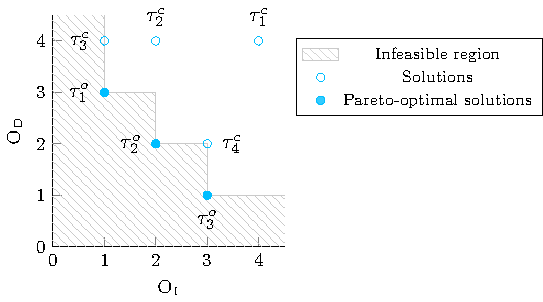
\includegraphics{biobj-inst.pdf}
  \end{minipage}
  \caption{Left: An example formula $\formula$ and two objectives $\Obj_\inc$ and $\Obj_\dec$.
    Right: the feasible region of $\formula$ in the objective space defined by $\Obj_\inc$ and $\Obj_\dec$.
    The solutions $\tau^o_1$ and $\tau^o_2$ (solid points) are Pareto-optimal, while $\tau^c_i$ for $i=1,\ldots,4$ are not.\label{fig:biobj-inst}}
\end{figure}

\begin{example}\label{ex:main}
  An example formula $\formula$ and two objectives $\Obj_\inc$ and $\Obj_\dec$ are shown on the left side in \cref{fig:biobj-inst}. 
  The solution space is illustrated on the right.
  The three solid dots correspond to the three Pareto points of $\formula$ w.r.t.\ $\Obj_\inc$ and $\Obj_\dec$. 
  Examples of Pareto-optimal solutions corresponding to these points are $\sol^o_1 = \soloone$, $\sol^o_2 = \solotwo$ and $\sol^o_3 = \solothree$.
  The solution $\sol^c_3 = \solcthree$ is dominated by $\sol^o_1$ ($\sol^o_1 \prec \sol^c_3$) because $\Obj_\inc(\sol^o_1) \leq \Obj_\inc(\sol^c_3)$ and $\Obj_\dec(\sol^o_1) < \Obj_\dec(\sol^c_3)$.
\end{example}

% Proposition: Ordered Pareto front
An important property of Pareto-optimal solutions to bi-objective problems is summarized by the next observation.
\begin{observation}[Adapted from~\autocite{DBLP:conf/aaai/HartertS14}] \label{obs:biobjective}
  Sorting the Pareto-optimal solutions of a bi-objective optimization problem under the objectives $\generalobj_1$ and $\generalobj_2$ w.r.t.\ increasing values of $\generalobj_1$ amounts to sorting them w.r.t.\ decreasing values of $\generalobj_2$ and vice-versa.
\end{observation}

% Example: Ordered Pareto front
\begin{example}
  Consider the formula $\formula$, the objectives $\Obj_\inc$ and $\Obj_\dec$ and the three Pareto-optimal solutions $\sol^o_1$, $\sol^o_2$ and $\sol^o_3$ from \cref{fig:biobj-inst} and \cref{ex:main}.
  By \cref{obs:biobjective}, sorting the Pareto-optimal solutions by decreasing value for one objective results in sorting them by increasing values for the other objective:
  we have $\Obj_\inc(\sol^o_1) = 1 < \Obj_\inc(\sol^o_2) = 2 < \Obj_\inc(\sol^o_3) = 3$ and $\Obj_\dec(\sol^o_1) = 3 > \Obj_\dec(\sol^o_2) = 2 > \Obj_\dec(\sol^o_3) = 1$.
\end{example}

\section{On Other Notions of Optimality\label{sec:other-notions}}

% Signposting
As mentioned in \cref{sec:multiopt}, Pareto optimality is only one---although a central---notion of optimality for multiple objectives.
Two other notions of optimality for bi-objective optimization that narrow down the set of solutions considered optimal are \emph{lexicographic optimization} and \emph{lexicographic max-ordering optimization}~\autocite{Ehrgott2005-5}.
These notions of optimality can be seen as a way of specifying in advance which Pareto-optimal solutions are of interest.
The solutions considered optimal are a subset of all Pareto-optimal solutions~\autocite{Ehrgott2005-5} and every algorithm finding all Pareto-optimal solutions will therefore also find all solutions optimal under these other notions.
For this reason, finding an optimal solution under these other notions of optimality can be considered easier than finding a representative solution for every Pareto point or enumerating all Pareto-optimal solutions.
Both lexicographic optimization and lexicographic max-ordering optimization are applicable for any number of objectives.
Here we describe them in the context of bi-objective optimization.

% Lexicographic optimization
In lexicographic optimization~\autocite{Ehrgott2005-5}, a preference over the objectives is enforced, considering only one of the ``end points'' of the Pareto front---i.e., a Pareto-optimal solution with the smallest value for the objective chosen as primary---optimal.
Formally, given a feasible set $\feasible$ and two objectives $\generalobj_1$ and $\generalobj_2$, a solution $x$ dominates another solution $x'$ in the lexicographic sense if (a)~$\generalobj_1(x) < \generalobj_1(x')$, or (b)~$\generalobj_1(x) = \generalobj_1(x')$ and $\generalobj_2(x) < \generalobj_2(x')$.
Intuitively, lexicographic optimization minimizes $\generalobj_1$, using $\generalobj_2$ as a tie-breaker.
The comparison criterion can also be seen as lexicographically comparing the string of objective values of two solutions, hence the name of the notion of optimality.

% Example: lexicographic optimization from a perspective of Pareto optimality
\begin{example}
  Consider again the formula $\formula$ and the objectives $\Obj_\inc$ and $\Obj_\dec$ from \cref{fig:biobj-inst}.
  Assume the objective $\Obj_\inc$ is chosen as the objective with higher priority.
  In this case, all solutions corresponding to the Pareto point $(3,1)$ (e.g., $\sol^o_1 = \soloone$) are lexicographically optimal.
\end{example}

% Lexicographic optimization with the weighted sum method
Lexicographic optimization can be cast into an optimization problem with a single objective with the help of the weighted sum method~\autocite{Ehrgott2005-3}.
This is a common approach to solving lexicographic optimization, since solving algorithms for optimization problems with one objective are widely available (e.g., MaxSAT~\autocite{handbook2-maxsat} or integer linear programming solvers~\autocite{ChenEtAl2010-intro}).

% Leximax optimization
Lexicographic max-ordering (leximax) optimization~\autocite{Ehrgott2005-5} is closely related to lexicographic optimization.
The difference between these two is that for leximax optimization, the objective values are sorted in descending order before comparing them lexicographically.
This leads to the Pareto points with the smallest maximum objective value being considered optimal.
Let $\generalobj_\text{max}(x) = \max\{\generalobj_1(x), \generalobj_2(x)\}$ and $\generalobj_\text{min}(x) = \min\{\generalobj_1(x), \generalobj_2(x)\}$.
Formally, a solution $x$ dominates another solution $x'$ in the leximax sense if (a)~$\generalobj_\text{max}(x) < \generalobj_\text{max}(x')$, or (b)~$\generalobj_\text{max}(x) = \generalobj_\text{max}(x')$ and $\generalobj_\text{min}(x) < \generalobj_\text{min}(x')$.
Informally speaking, this notion of optimality seeks to keep all objective values low by minimizing the maximum value first.
All leximax-optimal solutions are contained in the set of Pareto-optimal solutions.
However, they might correspond to different Pareto points.

% Example: lexicographic max-ordering optimization from a perspective of Pareto optimality
\begin{example}
  Consider again the formula $\formula$ and the objectives $\Obj_\inc$ and $\Obj_\dec$ in \cref{fig:biobj-inst}.
  The solution $\sol^o_2 = \solotwo$ is leximax-optimal since it has the smallest maximum objective value.
\end{example}

\section{Approaches to Bi-Objective Optimization\label{sec:approaches}}

% Signposting
In this section, we give an overview of earlier-proposed approaches to solving bi-objective optimization problems.
The focus here lies on \cref{sec:sat-based}, surveying SAT-based approaches.
In addition, we shortly survey exact approaches based on other declarative optimization paradigms, mainly constraint and mixed integer programming.
We conclude the section by giving a brief overview of inexact methods and discuss approaches that make use of different optimality definitions.

\subsection{SAT-Based Approaches\label{sec:sat-based}}

% Signposting
We highlight three key SAT-based approaches to bi-objective optimization under Pareto optimality:
enumeration of $P$-minimal solutions, enumeration of Pareto-minimal correction sets, and Seesaw.
Furthermore, we touch on SAT-based optimization under lexicographic optimality.

\subsubsection{$P$-Minimal Solution Enumeration\label{sec:p-minimal}}

% P-minimal solution enumeration
The approach perhaps closest to the one presented in this thesis reduces finding Pareto points to the enumeration of so-called $P$-minimal solutions~\autocites{DBLP:conf/cp/SohBTB17,DBLP:conf/ftp/KoshimuraNFH09}.
This approach was originally proposed for solving constraint satisfaction problems~\autocites{DBLP:reference/fai/2} encoded in CNF via the order encoding~\autocite{DBLP:conf/ictai/TamuraBS13}.
We note that the approach can be used with any encoding that allows for representing an objective value as a sorted unary number.
Here we present enumeration of $P$-minimal solutions using the totalizer encoding (recall \cref{sec:card-const}) instead of the order encoding as it also produces a unary representation of the objective values.

% The algorithm
Finding the Pareto points to the bi-objective optimization problem defined by $\formula$, $\Obj_1$ and $\Obj_2$ corresponds to enumerating the solutions of $\formula^\text{W} = \formula \land \tot(\Obj_1) \land \tot(\Obj_2)$ that are subset-minimal w.r.t.\ the outputs of the totalizers assigned to 0.
More precisely, if $P$ is the set of output literals of $\tot(\Obj_1) \land \tot(\Obj_2)$, then the goal is to enumerate solutions $\sol^m$ such that no other solution $\sol$ has $\{ l \mid l \in P, \sol(l) = 0 \} \subsetneq \{ l \mid l \in P, \sol^m(l) = 0 \}$.
The procedure for enumerating such solutions~\autocite{DBLP:conf/ftp/KoshimuraNFH09} works by
\begin{enumerate}[label=(\roman*)]
  \item using a solver to obtain any solution $\sol$ of $\formula^\text{W}$,
  \item iteratively minimizing the subset of variables of $P$ set to true by the solution, and,
  \item once a minimal solution $\sol^m$ has been found, adding the clause $(\ov{\Obj_{\inc}}{k_1} \lor \ov{\Obj_{\dec}}{k_2})$ containing the output variables corresponding to the lowest index set to true by $\sol_m$.
\end{enumerate}
We refer to the algorithm for enumerating $P$-minimal solutions as ``$P$-minimal'' for short.

% Example: P-minimal
\begin{example}\label{ex:pmin}
  Consider the formula $\formula$ and two objectives $\Obj_\inc$ and $\Obj_\dec$ from \cref{fig:biobj-inst}.
  $P$-minimal starts by building two totalizers $\tot(\Obj_\inc)$ and $\tot(\Obj_\dec)$ and invoking the SAT solver on $\formula^\text{W} = \formula \land \tot(\Obj_\inc) \land \tot(\Obj_\dec)$.
  The result is satisfiable;
  assume the first solution obtained is $\sol^c_1 = \solcone$.%
  \footnote{Note that the assignment of the auxiliary and output variables of the totalizer encoding are implied by the assignment of the input variables. For this reason we omit them when giving the assignment of a solution.} 
  In order to minimize $\sol^c_1$, the clause $(\ov{\Obj_\inc}{4} \lor \ov{\Obj_\dec}{4})$ is added to the SAT solver, and the solver is invoked again under the assumptions $\{ \ove{\Obj_\inc}{4}, \ove{\Obj_\dec}{4} \}$.
  The added clause blocks $\sol^c_1$ and all solutions dominated by $\sol^c_1$ from the search space.
  Assume the next solution obtained is $\sol^c_5 = \solmcstrap$. 
  Again, a clause $(\ov{\Obj_\inc}{3} \lor \ov{\Obj_\dec}{3})$ is added, and the SAT solver is queried with the assumptions $\{ \ove{\Obj_\inc}{3}, \ove{\Obj_\dec}{3} \}$.
  The result is \sat{};
  assume the solution obtained is $\sol^o_2 = \soloone$. 
  $P$-minimal then adds the clause $(\ov{\Obj_\inc}{2} \lor \ov{\Obj_\dec}{2})$ and invokes the solver again under the assumptions $\{ \ove{\Obj_\inc}{2}, \ove{\Obj_\dec}{2} \}$.
  The result is \unsat{} which proves that $\sol^o_2$ is Pareto-optimal. 
  To find a next Pareto-optimal solution, the solver is queried without any assumptions for a new solution to start the minimization process from.
\end{example}

% Extending P-minimal to enumerate the full Pareto front
As presented in~\autocite{DBLP:conf/cp/SohBTB17}, $P$-minimal enumerates a single representative solution per Pareto point.
It can, however, be extended to enumerating all Pareto-optimal solutions by adding a relaxation variable to the clause added at each iteration and iteratively blocking solutions once they have been proven to be Pareto-optimal.
More details on this are given later on \cref{sec:competing}.

\subsubsection{Enumeration of Pareto-Minimal Correction Sets\label{sec:pareto-mcs}}

% Pareto MSCes
An approach for computing Pareto-optimal solutions via so-called Pareto-minimal correction sets (ParetoMCSes) has been previously proposed~\autocite{DBLP:conf/ijcai/Terra-NevesLM18a,DBLP:conf/aaai/Terra-NevesLM18,DBLP:conf/ijcai/Terra-NevesLM18}.
A ParetoMCS (w.r.t.\ two objectives $\Obj_1$ and $\Obj_2$) consists of two sets of literals $(M_1, M_2)$ such that (i)~$M_1 \subset \Obj_1$ and $M_2 \subset \Obj_2$, and (ii)~there is a Pareto-optimal solution $\sol$ that sets $\sol(l) = 1$ for all $l \in M_1 \cup M_2$ and $\sol(l) = 0$ for all other $l \in (\Obj_1 \cup \Obj_2) \setminus (M_1 \cup M_2)$.
Computing Pareto-optimal solutions can be reduced to the computations of ParetoMCSes~\autocite{DBLP:conf/ijcai/Terra-NevesLM18a}.
The task of computing ParetoMCSes is accomplished by enumerating all subsets $T \subset  (\Obj_1 \cup \Obj_2)$ for which (i)~$\formula \land \bigwedge_{l \in  (\Obj_1 \cup \Obj_2) \setminus T} (\lnot l)$ is satisfiable, and (ii)~$\formula \land \bigwedge_{l \in  (\Obj_1 \cup \Obj_2) \setminus T'} (\lnot l)$ is unsatisfiable for all $T' \subsetneq T$.
Let $\mathcal{T}$ be the collection of all such sets.
The Pareto-optimal solutions are obtained by extracting the solutions satisfying $\formula \land \bigwedge_{l \in  (\Obj_{\inc} \cup \Obj_\dec) \setminus T} (\lnot l)$ for all $T \in \mathcal{T}$ and removing the dominated ones~\autocite{DBLP:conf/ijcai/Terra-NevesLM18a}.
The computation of $\mathcal{T}$ corresponds to enumeration of minimum correction sets, to which numerous algorithms have been proposed~\autocites{DBLP:conf/lpar/BendikC20,DBLP:conf/hvc/MorgadoLM12,DBLP:conf/sat/PrevitiMJM17}.
The ParetoMCS approach to multi-objective optimization is approximative in that it can only guarantee that a solution is Pareto-optimal once the full set $\mathcal{T}$ has been computed.

% Example: A MCS that is not Pareto-optimal
\begin{example}\label{ex:MCS}
  Consider the formula $\formula$ and two objectives $\Obj_\inc$ and $\Obj_\dec$ from \cref{fig:biobj-inst}.
  The ParetoMCS enumeration procedure will return the solution $\sol = \solmcstrap$ since no solution $\sol'$ of $\formula$ has $\{l \in \Obj_\inc \cup \Obj_\dec \mid  \sol'(l) = 1\} \subsetneq \{i_1, i_3, i_4, d_1, d_3, d_4\}$.
  The solution $\sol$ is not Pareto-optimal, but only filtered out when a solution that dominates it is enumerated.
  However, there are no guarantees on when such a dominating solution is found. 
\end{example}

% Naming
We will refer to this algorithm for enumerating Pareto-optimal solutions via enumerating ParetoMCSes as ``ParetoMCS'' for short.

\subsubsection{Implicit Hitting Set Approach: Seesaw\label{sec:seesaw}}

% Implicit hitting set approach
The implicit hitting set approach~\autocites{DBLP:conf/soda/ChandrasekaranKMV11,DBLP:journals/ior/Moreno-CentenoK13,DBLP:journals/amai/ParkerR96,DBLP:journals/ijmms/ReggiaNW83,DBLP:journals/ai/Reiter87} has, among other formalisms and problems, been successfully applied to MaxSAT~\autocite{DBLP:conf/cp/DaviesB13,DBLP:conf/sat/DaviesB13,DBLP:conf/cp/DaviesB11,DBLP:conf/sat/BergBP20} and other SAT-related applications~\autocite{DBLP:conf/ecai/IgnatievMM16,DBLP:conf/cp/IgnatievPLM15,DBLP:conf/kr/SaikkoWJ16}.
Recently, Seesaw~\autocite{DBLP:conf/cp/JanotaMSM21} was proposed as a generalized implicit hitting set framework for bi-objective optimization.
The overarching idea is that an optimization problem is modelled as a set $\cores$ of so-called \emph{cores} which represent an undesirable or conflicting substructure of the problem.
Note that these cores are not necessarily equal to a core in SAT solving as described in \cref{sec:inc-sat};
for this reason, we will be referring to them as \emph{optimization cores} from now on.
For multiple objectives, an optimization core is only equivalent to a core if the decreasing objective is constrained to not be worse than the last value.
In contrast to our work, in Seesaw one of the objectives is treated as a black box.
This black box view does, however, also allow for SAT-based instantiations of Seesaw.

% Seesaw in a SAT context
In our context the Seesaw algorithm computes Pareto-optimal solutions of a formula $\formula$ w.r.t.\ $\Obj_\inc$ and $\Obj_\dec$ by maintaining a collection $\cores$ of optimization cores that are subsets of $\Obj_\inc$.
Informally speaking, in the bi-objective setting, every solution $\sol$ that improves on $\Obj_\dec$ needs to assign at least one literal from each core to 1.
The algorithm works iteratively by computing a hitting set $\hs \subset \Obj_\inc$ (using an integer programming solver), i.e., a subset-minimal set of literals of $\Obj_\inc$ that intersects with each optimization core in $\cores$.
Next, a solution $\sol$ is computed, so that $\sol(l) = 1$ for each $l \in \hs$, $\sol(l) = 0$ for each $l \in \Obj_\inc \setminus \hs$, and $\Obj_\dec(\sol)$ is the smallest possible value for all such solutions if one exists.
This is the step which employs a SAT solver in our instantiations of the algorithm.
Seesaw then extracts a new core that $\hs$ does not intersect with.
The Pareto-optimal solutions of $\formula$ are identified by the size of the hitting set increasing.
More precisely, if the hitting set is found to increase from size $|\hs|$ to size $|\hs_2|$ with $|\hs_2|>|\hs|$, the solution $\sol$ found with a hitting set of size $|\hs|$ that has the smallest minimum value $\Obj_\dec(\sol)$ is Pareto-optimal~\autocite{DBLP:conf/cp/JanotaMSM21}.

% Example: Seesaw
\begin{example}
  Consider the formula $\formula$ and two objectives $\Obj_\inc$ and $\Obj_\dec$ from \cref{fig:biobj-inst}. 
  Initially, there are no optimization cores, so $\cores = \emptyset$ and $\hs = \emptyset$.
  Since there is no $\sol$ that sets $\sol(l) = 0$ for each $l \in \Obj_\inc$, the iteration ends by extracting the optimization core $\Obj_\inc$. 
  The intuition is, that any solution $\sol$ of $\formula$ sets at least one variable in $\Obj_\inc$ to 1.
  In the next iteration, a minimum hitting set over $\cores = \{ \Obj_\inc \}$ is computed.
  There are a number of alternatives;
  assume $\hs = \{ i_1 \}$.
  Since there is no $\sol$ that sets $\sol(i_2) = \sol(i_3) = \sol(i_4) = 0$, the iteration ends with extracting the optimization core $\{ i_2, i_3, i_4\}$.
  The same intuition as earlier holds for this core.
  Assume the next hitting set computed is $\hs = \{i_2\}$.
  Now there is a $\sol$ that sets $\sol(i_1) = \sol(i_3) = \sol(i_4) = 0$;
  one that also minimizes $\Obj_\dec(\sol)$ is $\sol^o_1 = \soloone$.
  The iteration ends with extracting the optimization core $\core = \{i_1, i_3, i_4\}$.
  Now the intuition is that, since $\sol^o_1$ minimizes $\Obj_\dec$ over solutions that assign $\sol(l) = 0$ for every $l \notin \hs$, every solution that obtains a lower value of $\Obj_\dec$ assigns at least one literal of $\core$ to 1. 
  Assume next we get $\hs = \{i_3\}$ for which no corresponding solution exists;
  the optimization core $\{i_1, i_2, i_4\}$ is added to $\cores$.
  Now we have $\cores = \{ \Obj_\inc, \{i_2, i_3, i_4\}, \{i_1, i_3, i_4\}, \{i_1, i_2, i_4\}\}$;
  the only minimum hitting set is $\hs = \{ i_4 \}$.
  There is no $\sol$ that sets $\sol(i_1) = \sol(i_2) = \sol(i_3) = 0$ so a new optimization core $\{i_1, i_2, i_3\}$ is extracted. 
  Next, one possible hitting set is $\hs = \{i_1, i_3\}$.
  Since the size of the hitting set grew from 1 to 2, the algorithm concludes that $\sol^o_1$ is Pareto-optimal. 
  The algorithm continues in this manner, finding the Pareto-optimal $\sol^o_2$ and $\sol^o_3$ in the process.
  After computing the hitting set consisting of all literals in $\Obj_\inc$, the core extracted is $\emptyset$ at which point the algorithm terminates. 
\end{example}

% Core extraction strategies for Seesaw
Note that the optimization core extraction strategy that only computes $\Obj_\inc \setminus \hs$ as the new optimization core detailed in the example corresponds to what is called the weakest possible strategy in the original paper~\autocite{DBLP:conf/cp/JanotaMSM21}.
Seesaw is only feasible in practice when using a stronger optimization core extraction strategy since Seesaw otherwise reduces to enumerating all subsets of $\Obj_\inc$ as hitting sets~\autocite{DBLP:conf/cp/JanotaMSM21}.
One such stronger strategy for extracting optimization cores that is generally applicable if the oracle function is anti-monotone was presented in the original paper~\autocite{DBLP:conf/cp/JanotaMSM21}.
When using a SAT-based instantiation of the black box objective in Seesaw, it is also possible to use cores extracted by the SAT solver as the optimization cores for Seesaw.
More details on this are given with the concrete instantiations of Seesaw that we implement in \cref{sec:competing}.

% Extending Seesaw to full pareto front enumeration
Also note that, in contrast to \algname{} and $P$-minimal, extending Seesaw as it was originally presented~\autocite{DBLP:conf/cp/JanotaMSM21} to support the enumeration of all Pareto-optimal solutions seems non-trivial.
For a non-formal intuition note that, while Seesaw is guaranteed to find at least one solution obtaining the objective values of each Pareto point, the non-deterministic hitting set computation might steer the algorithm past other solutions that obtain the same values.

\subsubsection{SAT-Based Lexicographic Optimization\label{sec:lex-opt}}

% (SAT-based) lexicographic optimization
There is also earlier work on SAT-based lexicographic optimization (recall \cref{sec:other-notions})~\autocites{DBLP:journals/ors/EhrgottG00,DBLP:conf/ijcai/ArgelichLS09,DBLP:journals/amai/Marques-SilvaAGL11}. 
% Lexicographic optimization and MaxSAT
Lexicographic optimization is closely related to the so-called multi-level optimization problem.
In particular, both can be cast as single-objective optimization and solved with a MaxSAT solver~\autocites{DBLP:conf/ijcai/ArgelichLS09,DBLP:journals/amai/Marques-SilvaAGL11}.
In fact, many modern MaxSAT solvers exploit multilevel properties of input instances in order to improve search efficiency~\autocites{DBLP:conf/vmcai/PaxianRB21,DBLP:conf/cp/AnsoteguiBGL12}.

\subsection{Other Declarative Optimization Paradigms\label{sec:other-approaches}}

% CP-based approaches
Beyond SAT-based approaches, multi-objective optimization has been studied in the context of other declarative optimization paradigms.
An early algorithm that can be used in constraint programming~\autocite{DBLP:reference/fai/2} is based on the lexicographic method~\autocite{Wassenhove1980}.
A branch-and-bound-based algorithm that outperforms the previous algorithm was presented later~\autocite{DBLP:conf/ecai/Gavanelli02}.
This improved filtering algorithm was improved again by the Pareto constraint~\autocite{DBLP:conf/cp/SchausH13,DBLP:conf/aaai/HartertS14}.
The resulting search algorithm is similar to ParetoMCS in that it maintains a set $\mathcal{T}$ of solutions that do not dominate each other.
When a new solution is found, any solution it dominates is removed from $\mathcal{T}$.

% CP-based leximax optimization
Other than approaches for finding all Pareto-optimal solutions, there have also been constraint programming algorithms proposed for finding leximax-optimal solutions.
In~\autocite{DBLP:journals/ai/BouveretL09}, five algorithms for this problem are given.
There is one branch-and-bound-based algorithm and another algorithm based on adding constraints to encode the sorted objective value vector, minimizing multiple times over that.

% MIP-based approaches
Multi-objective optimization has also been studied in the context of linear programming, mixed integer programming and zero-one-programming~\autocites{Ehrgott2005-6,Rasmussen1986,DBLP:journals/eor/AlvesC07}.
There are different algorithmic approaches in this field, some based on the Simplex algorithm~\autocites{Ehrgott2005-7,DBLP:journals/mp/EvansS73}, others on branch-and-bound~\autocites{Adelgren2021,DBLP:journals/siamjo/SantisENR20} while a last category build on reducing the problem of finding a Pareto-optimal solution to single-objective mixed integer programming~\autocites{DBLP:journals/jota/Sun17,DBLP:journals/ol/LuMS20,Soland1979}.

\subsection{Inexact Approaches\label{sec:approximative}}

% Inexact vs. exact methods
Other than the exact algorithms, there are also inexact search algorithms for multi-objective optimization problems~\autocite{Saini2021}.
These algorithms are \emph{not} guaranteed to return the exact Pareto front, but they will return approximately optimal solutions.
Depending on the application, such an approximate solution might be sufficient.
Inexact algorithms are mainly used for problems that are too large to solve them with exact methods under given resource constraints.

% Examples of ineaxact algorithms
Literature on inexact optimization algorithms is vast, for a survey see~\autocite{Saini2021}.
Two important categories or algorithms that have been extended to multiple objectives are simulated annealing~\autocites{DBLP:journals/science/KirkpatrickGV83,DBLP:journals/tec/BandyopadhyaySMD08,DBLP:journals/isci/SenguptaS18} and evolutionary algorithms~\autocites{DBLP:books/daglib/0087893,DBLP:journals/jgo/StornP97,DBLP:journals/tec/DebAPM02}.
Both of these categories of algorithms can be described as ``local search style'', where one or more solutions are iteratively modified to find better solutions.